%%%%%%%%%%%%%%%%%%%%%%%%%%%%%%%%%%%%%%%%%%%%%%%%%%%%%%%%%%%%%%%%%%%%%%%%%%%%%%%%
%%% Homework Two -- Latex Template:
%%% Tested against the pdflatex compiler
%%%

\documentclass[english]{article}

%%%%%%%%%%%%%%%%%%%%%%%%%%%%%%%%%%%%%%%%%%%%%%%%%%%%%%%%%%%%%%%%%%%%%%%%%%%%%%%%
%%% Document Preamble
%%% - contains the external content (packages) and formatting settings
%%% - modification should be unnecessary unless you want to add additional
%%%   functionality or change the aesthetics

%%% Hyperref: insert links
% See: https://www.overleaf.com/learn/latex/Hyperlinks
\usepackage[unicode=true]{hyperref}

%%% Hyperref: links should appear blue as you would expect
\hypersetup{
  colorlinks=true,
  linkcolor=blue,
  urlcolor=blue,
  filecolor=blue,
}

\usepackage [margin=1.0in] {geometry}

%%% Listings: use to include code in your solutions
% See: https://www.overleaf.com/learn/latex/Code_listing
\usepackage{listings}

%%% Listings: setup defaults for code formatting
\lstset{
  language={C++},
  frame=tb,
  numbers=left,
  numberstyle=\tiny,
  basicstyle=\small\sffamily,
  breaklines=true,
}

%%% GraphicX: insert images (e.g. screenshots) into the document
% See: https://www.overleaf.com/learn/latex/Inserting_Images
\usepackage{graphicx}

%%% Float: Allows the use of the H specifier in images to force them in place
\usepackage{float}


%%% Enumitem: alphabetic enumerations with improved syntax
% E.g.
% (a) ...
% (b) ...
\usepackage[shortlabels]{enumitem}


%%% AMS Math: access to math environments alike align
% Aligning: https://www.overleaf.com/learn/latex/Aligning_equations_with_amsmath 
\usepackage{amsmath}

% Additional options when using tables
\usepackage{array}

%%% Custom commands

\newcounter{problemi}
\setcounter{problemi}{1}

\newcommand*{\headfont}{\fontsize{1.1em}{1.0em}\selectfont}


\newcommand\problem[1]{
  \noindent{\headfont\\\theproblemi. #1}\\
  \stepcounter{problemi}\smallskip
}

\newcommand*{\code}[1]{\texttt{#1}}


\begin{document}

%%%%%%%%%%%%%%%%%%%%%%%%%%%%%%% COVER PAGE %%%%%%%%%%%%%%%%%%%%%%%%%%%%%%%%%%%%%

\begin{centering}
    {\Large CSCE 221 Cover Page} \\ \medskip    
\end{centering}

Please list all sources in the table below including web pages which you used to solve or implement the current homework. If you fail to cite sources you can get a lower number of points or even zero, read more Aggie Honor System Office \url{https://aggiehonor.tamu.edu/} \\

% EDIT: the below information appropriately
\noindent
\begin{center}
    {\large
    \begin{tabular}{|p{0.35\linewidth}|p{0.45\linewidth}|} \hline
        Name          & Clayton Kristiansen         \\ \hline
        UIN           & 328003173         \\ \hline
        Email address & kristiansenc@tamu.edu      \\ \hline
    \end{tabular}
    }
\end{center}

Cite your sources using the table below. Interactions with TAs and resources presented in lecture do not have to be cited.
\noindent
\begin{center}
    {\large
    \begin{tabular}{|>{\centering\arraybackslash}m{0.25\linewidth}|m{0.70\textwidth}|} \hline
        {\large People}            &
            \begin{enumerate}
                % EDIT
                % People: Add sources below as items
                \item None
            \end{enumerate}
        \\ \hline
        {\large Webpages}          & 
            \begin{enumerate}
                % EDIT
                % Webpages: Add sources below as items
                \item None
            \end{enumerate}
        \\ \hline
        {\large Printed Materials} &
            \begin{enumerate}
                % EDIT
                % Printed Material: Add sources below as items
                \item None
            \end{enumerate}
        \\ \hline
        {\large Other Sources}     &
            \begin{enumerate}
                % EDIT
                % Other sources: Add sources below as items
                \item None
            \end{enumerate}
        \\ \hline
    \end{tabular}
    }
\end{center}

\pagebreak

%%%%%%%%%%%%%%%%%%%%%%%%%%%%%%% HOMEWORK TWO %%%%%%%%%%%%%%%%%%%%%%%%%%%%%%%%%%%%%

\begin{centering}
    {\Huge Homework 2}\\ \bigskip
    {\Large Due March 25 at 11:59 PM}\\ \bigskip
\end{centering}

\textbf{Typeset your solutions to the homework problems preferably in \LaTeX or LyX.
See the class webpage for information about their installation and tutorials.}

%%%%%%%%%%%%%%%%%%%%%%%%%%%%%%%%% PROBLEM 1 %%%%%%%%%%%%%%%%%%%%%%%%%%%%%%%%%%%%%%%

\problem{(15 points)
Provided two sorted lists, \code{l1} and \code{l2}, write a function in C++ to \emph{efficiently} compute \code{l1 $\cap$ l2} using only the basic STL list operations. The lists may be empty or contain a different number of elements e.g $|\code{l1}| \neq |\code{l2}|$. You may assume \code{l1} and \code{l2} will not contain duplicate elements.
}

\noindent Examples (all set members are list node):
\begin{itemize}
  \item $\{1, 2, 3, 4\} \cap \{2, 3\} = \{2, 3\}$
  \item $\emptyset \cap \{2, 3\} = \emptyset$
  \item $\{2, 9, 14\} \cap \{1, 7, 15\} = \emptyset$
\end{itemize}

\bigskip

\begin{enumerate}[(a)]
  \item Complete the function below. Do not use any routines from the algorithm header file.

\begin{lstlisting}
#include <list>

std::list<int> intersection(const std::list<int> & l1, const std::list<int> & l2) 
{
    std::list<int> l3;
    
    std::list<int>::const_iterator el1 = l1.begin();
    std::list<int>::const_iterator el2 = l2.begin();

    while(el1 != l1.end())
    {
        el2 = l2.begin();
        while(el2 != l2.end())
        {
            if(*el1 == *el2)
            {
                l3.push_back(*el1);
            }
            el2++;
        }
        el1++;
    }

    return l3;
}
\end{lstlisting}

  \item Verify that your implementation works properly by writing two test cases. Provide screenshot(s) with the results of your testing.

\begin{lstlisting}
int main()
{
    std::list<int> l1;
    std::list<int> l2;
    l1.push_back(2);
    l1.push_back(3);
    l1.push_back(7);
    l1.push_back(8);
    l1.push_back(6);
    l2.push_back(1);
    l2.push_back(2);
    l2.push_back(3);
    l2.push_back(7);
    std::cout << "TEST CASE 1:\n";
    intersection(l1, l2);
    l1.clear();
    l2.clear();
    l1.push_back(1);
    l1.push_back(2);
    l1.push_back(3);
    l1.push_back(4);
    l1.push_back(5);
    l1.push_back(6);
    l1.push_back(7);
    l1.push_back(7);
    l1.push_back(8);
    l1.push_back(10);
    l2.push_back(5);
    l2.push_back(4);
    l2.push_back(3);
    l2.push_back(8);
    std::cout << "\n\n\nTEST CASE 2:\n";
    intersection(l1, l2);
}
\end{lstlisting}

  \begin{figure}[H]
     \centering
     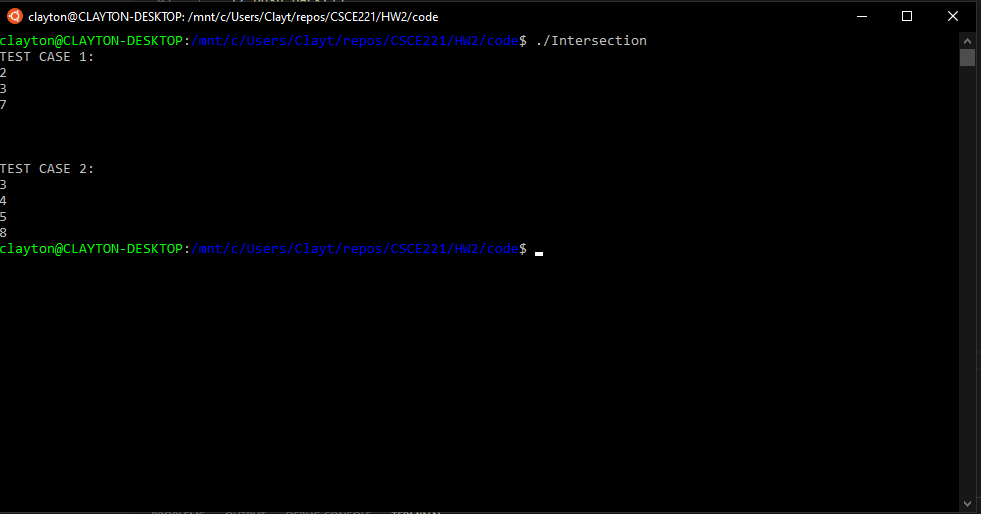
\includegraphics[width=0.8\linewidth]{1-tests.png}
     \caption{Results of testing the \code{intersection} function}%
     \label{fig:intersection_tests}
  \end{figure}  

  \item What is the running time of your algorithm? Provide a big-O bound. Justify.

  \begin{equation}
    f(n) \in O(n^2)
  \end{equation}
  
  Assuming n is the max of the two set sizes:
  % You may also want a derivation in your justification
  \begin{align}
    f(n) &= 3n^2 + 3n + 3 \\
         &= n^2
  \end{align}

\end{enumerate}

%%%%%%%%%%%%%%%%%%%%%%%%%%%%%%%%% PROBLEM 2 %%%%%%%%%%%%%%%%%%%%%%%%%%%%%%%%%%%%%%%

\problem{(15 points)
  Write a C++ recursive function that counts the number of nodes in a singly linked list. Do not modify the list.
}

Examples:
\begin{itemize}
  \item \code{count\_nodes($ (2) \rightarrow (4) \rightarrow (3) \rightarrow \text{nullptr}$)} = 3
  \item \code{count\_nodes($\text{nullptr}$)} = 0
\end{itemize}

\bigskip

\begin{enumerate}[(a)]
  \item Complete the function below:
  \label{enum:recursive_node_imp}

\begin{lstlisting}
template <typename T>
struct Node
{
    Node *next;
    T obj;

    Node(T obj, Node *next = nullptr)
        : obj(obj), next(next)
    { }
};

template <typename T>
int count_nodes(Node<T>* n)
{
    while(n->next != nullptr)
    {
        return 1 + count_nodes(n->next);
    }
    return 1;
}
\end{lstlisting}

  \item Verify that your implementation works properly by writing two test cases for the function you completed in part \ref{enum:recursive_node_imp}. Provide screenshot(s) with the results of your testing.

\begin{lstlisting}
int main()
{
    Node<int>* n1 = new Node<int>(0);
    Node<int>* first = n1;
    n1->next = new Node<int>(4); n1 = n1->next;
    n1->next = new Node<int>(3); n1 = n1->next;
    n1->next = new Node<int>(6); n1 = n1->next;
    n1->next = new Node<int>(2); n1 = n1->next;
    n1->next = new Node<int>(7); n1 = n1->next;
    n1->next = new Node<int>(8); n1 = n1->next;
    n1->next = new Node<int>(1);

    std::cout << "First Test:\n\nSize: ";
    std::cout << count_nodes<int>(first);


    Node<int>* n2 = new Node<int>(0);
    first = n2;
    n2->next = new Node<int>(2); n2 = n2->next;
    n2->next = new Node<int>(5); n2 = n2->next;
    n2->next = new Node<int>(68); n2 = n2->next;
    n2->next = new Node<int>(232); n2 = n2->next;
    n2->next = new Node<int>(713241534); n2 = n2->next;
    n2->next = new Node<int>(86); n2 = n2->next;
    n2->next = new Node<int>(0); n2 = n2->next;
    n2->next = new Node<int>(1); n2 = n2->next;
    n2->next = new Node<int>(2); n2 = n2->next;
    n2->next = new Node<int>(3); n2 = n2->next;
    n2->next = new Node<int>(12);

    std::cout << "\n\n\n\nSecond Test:\n\nSize: ";
    std::cout << count_nodes<int>(first) << "\n";
}
\end{lstlisting}

\begin{figure}[H]
    \centering
    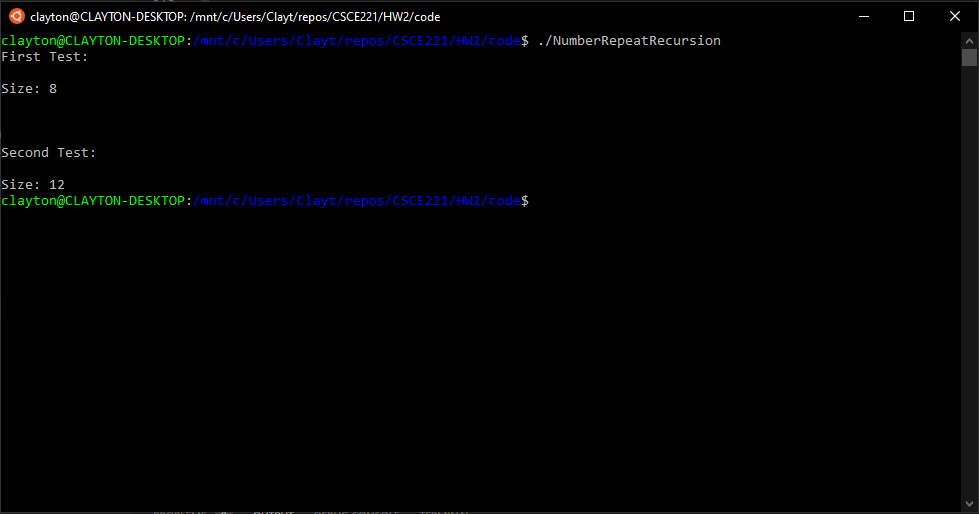
\includegraphics[width=0.8\linewidth]{2-tests.png}
    \caption{Results of testing the \code{count nodes} function}
    \label{fig:intersection_tests}
 \end{figure}  

  \item Write a recurrence relation that represents your algorithm.
  
  \begin{equation}
    T(n) = \begin{cases}
      T(n - 1) + O(1), & \text{if } n > 1 \\
      O(1), & \text{if } n = 1
    \end{cases} 
  \end{equation}
  \begin{equation}
    T(0) = 1
  \end{equation}

  \item Solve the recurrence relation using the iterating or recursive tree method to obtain the running time of the algorithm in Big-O notation.

  You may want to embed an image. If so, use a figure code block.
  \begin{align}
    T(n) &= T(n - 1) + O(1) \\
         &= T(n - 2) + 2 * O(1) \\
         &= T(n - 3) + 3 * O(1) \\
         &= T(n - 4) + 4 * O(1) \\
         &\cdots \\
         &= T(n - n) + n * O(1) \\ 
         &= T(0) + n * O(1) \\
         &= 1 + n * O(1) \\
         &= O(n) 
  \end{align}

\end{enumerate}

%%%%%%%%%%%%%%%%%%%%%%%%%%%%%%%%% PROBLEM 3 %%%%%%%%%%%%%%%%%%%%%%%%%%%%%%%%%%%%%%%

\problem{(15 points)
  Write a C++ recursive function that finds the maximum value in an array 
  (or vector) of integers \emph{without} using any loops. You may assume the
  array will always contain at least one integer. Do not modify the array.
}

\begin{enumerate}[(a)]
  \item Complete the function below:

\begin{lstlisting}
#include <iostream>
#include <vector>

using std::vector;

int find_max_value(vector<int> v, int index = 0)
{
    if(index + 1 >=  v.size())
    {
        return v[index];
    }
    int val = find_max_value(v, ++index);
    if(val > v[index])
    {
        return val;
    }
    return v[index];
}
\end{lstlisting}

  \item Verify that your implementation works properly by writing two test cases. Provide screenshot(s) with the results of the tests.

\begin{lstlisting}
int main()
{
    std::vector<int> vec;
    vec.push_back(12);
    vec.push_back(21);
    vec.push_back(3);
    vec.push_back(234);
    vec.push_back(3);
    vec.push_back(12);
    vec.push_back(7);
    vec.push_back(1);
    vec.push_back(2);

    std::cout << "First Test:\n\nSize: ";
    std::cout << find_max_value(vec);

    vec.clear();
    vec.push_back(1);
    vec.push_back(2);
    vec.push_back(3);
    vec.push_back(4);
    vec.push_back(5);
    vec.push_back(6);
    vec.push_back(7);
    vec.push_back(8);
    vec.push_back(9);

    std::cout << "\n\n\n\nSecond Test:\n\nSize: ";
    std::cout << find_max_value(vec) << "\n";
}
\end{lstlisting}

  \begin{figure}[H]
    \centering
    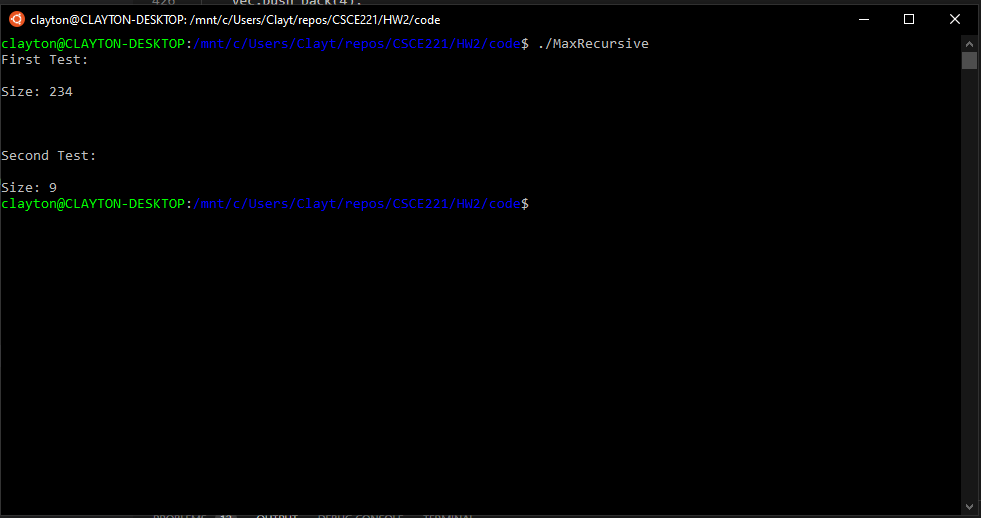
\includegraphics[width=0.8\linewidth]{3-test.png}
    \caption{Results of testing the \code{find\_max\_value} function}%
    \label{fig:find_max_value}
  \end{figure}  

  \item Write a recurrence relation that represents your algorithm.

  \begin{equation}
    T(n) = \begin{cases}
      T(n - 1) + O(1), & \text{if } n > 1 \\
      O(1), & \text{if } n = 1
    \end{cases}
  \end{equation}

  \item Solve the recurrence relation and obtain the running time of the algorithm in Big-O notation. Show your process.

  You may want to embed an image. If so, use a figure code block.
  \begin{align}
    T(n) &= T(n - 1) + O(1) \\
         &= T(n - 2) + 2 * O(1) \\
         &= T(n - 3) + 3 * O(1) \\
         &= T(n - 4) + 4 * O(1) \\
         &\cdots \\
         &= T(n - n) + n * O(1) \\ 
         &= T(0) + n * O(1) \\
         &= 1 + n * O(1) \\
         &= O(n) 
  \end{align}

\end{enumerate}

%%%%%%%%%%%%%%%%%%%%%%%%%%%%%%%%% PROBLEM 4 %%%%%%%%%%%%%%%%%%%%%%%%%%%%%%%%%%%%%%%

\problem{(15 points) 
  What is the best, worst and average running time of quick sort algorithm?
}

Best case: 
\begin{equation}
    O(nlog(n))
  \end{equation}
Average case: 
\begin{equation}
    O(nlog(n))
  \end{equation}
Worst case: 
\begin{equation}
    O(n^2)
  \end{equation}

\begin{enumerate}[(a)]
  % QUESTION: Do they need to solve them?
  \item Provide recurrence relations. For the average case, you may assume that quick sort partitions the input into two halves proportional to $c$ and $1 - c$ on each iteration.
  \label{enum:recurrence_relation}

  Best:
  \begin{equation}
    T(n) = \begin{cases}
      2T(n/2) + O(n), & \text{if } n > 1 \\
      0, & \text{if } n = 1
    \end{cases}
  \end{equation}

  Average:
  \begin{equation}
    T(n) = \begin{cases}
      T(cn) + T((1 - c)n) + n, & \text{if } n > 1 \\
      0, & \text{if } n = 1
    \end{cases}
  \end{equation}
  
  Worst:
  \begin{equation}
    T(n) = \begin{cases}
      T(n-1) + n, & \text{if } n > 1 \\
      0, & \text{if } n = 1
    \end{cases}
  \end{equation}

  \item Solve each recurrence relation you provided in part \ref{enum:recurrence_relation}

  % You may want to include an image using the figure environment and solve it on paper
  % You could also use the align environment to typeset math
  \begin{figure}[H]
    \centering
    \includegraphics[width=1.0\linewidth]{Best.jpg}
    \caption{Solution to best case recurrence relation}%
    \label{fig:recurrence_solution}
  \end{figure} 
  \begin{figure}[H]
    \centering
    \includegraphics[width=1.0\linewidth]{Average.jpg}
    \caption{Solution to average case recurrence relation}%
    \label{fig:recurrence_solution}
  \end{figure}  
  \begin{figure}[H]
    \centering
    \includegraphics[width=1.0\linewidth]{Worst.jpg}
    \caption{Solution to worst case recurrence relation}%
    \label{fig:recurrence_solution}
  \end{figure}  

  \item Provide an arrangement of the input array which results in each case. Assume the first item is always chosen as the pivot for each iteration.

    \begin{table}[H]
      \centering
      \begin{tabular}{c c}
        Best    & $\{5, 2, 3, 4, 1, 7, 8, 9, 6\}$ \\
        Average & $\{9, 6, 7, 4, 5, 8, 3, 1, 2\}$ \\
        Worst   & $\{1, 2, 3, 4, 5, 6, 7, 8, 9\}$ 
      \end{tabular}
    \end{table}

\end{enumerate}

%%%%%%%%%%%%%%%%%%%%%%%%%%%%%%%%% PROBLEM 5 %%%%%%%%%%%%%%%%%%%%%%%%%%%%%%%%%%%%%%%

\problem{(15 points)
  Write a C++ function that counts the total number of nodes with two children in a 
  binary tree (do not count nodes with one or none child). You can use a STL container 
  if you need to use an additional data structure to solve this problem. 
}
\begin{figure}[H]
  \centering
  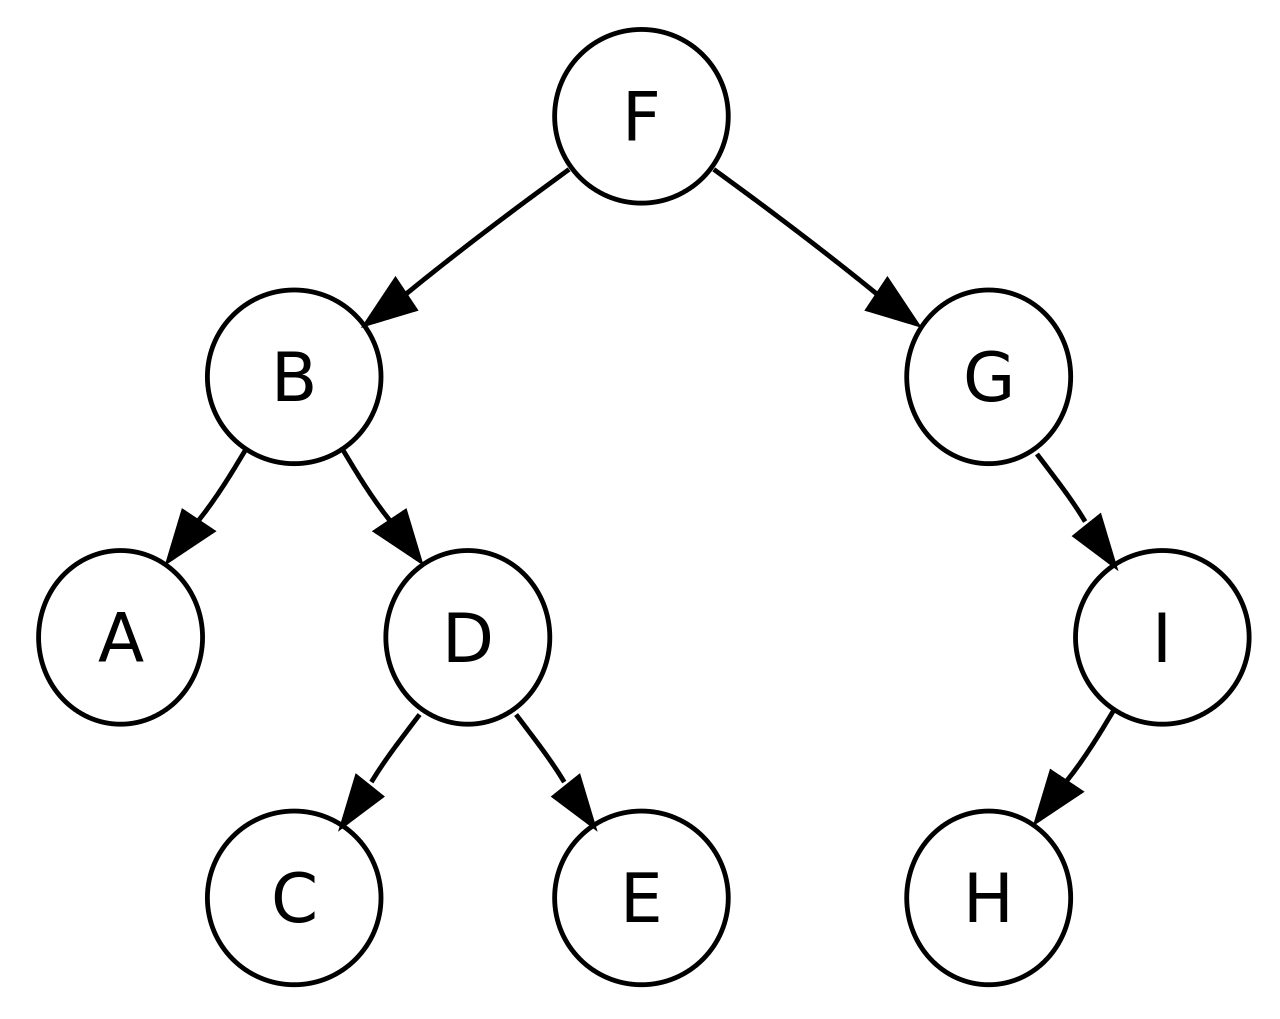
\includegraphics[width=0.3\linewidth]{./binary_tree_example.png}
  \caption{Calling \code{count\_filled\_nodes} on the root node F returns \code{3}}%
  \label{fig:binary_tree_example}
\end{figure}

\begin{enumerate}[(a)]
  \item Complete the function below. The function will be called with the root node (e.g. \code{count\_filled\_nodes(root)}). The tree may be empty. Do not modify the tree.

\begin{lstlisting}
#include <vector>

template<typename T>
struct Node {
  Node<T> *left, *right;
  T obj;

  Node(T obj, Node<T> * left = nullptr, Node<T> * right = nullptr)
    : obj(obj), left(left), right(right)
  { }
};

template <typename T>
int count_filled_nodes(const Node<T> *node)
{
    if(node->left != nullptr && node->right != nullptr)
    {
        int numNodes = 0;
        numNodes += count_filled_nodes(node->left);
        numNodes += count_filled_nodes(node->right);
        return 1 + numNodes;
    }
    else
    {
        if(node->left != nullptr)
        {
            return count_filled_nodes(node->left);
        }
        else if(node->right != nullptr)
        {
            return count_filled_nodes(node->right);
        }    
    }
    return 0;
}

\end{lstlisting}

  \item Use big-O notation to classify your algorithm. Show how you arrived at your answer.

  \begin{equation}
    f(n) \in O(n)
  \end{equation}
  The recursive function visits each node in the tree once to determine whether any node has two existing children. 
  This is a simple Preorder Traversal algorithm where the status of the current node's children are determined, 
  then the left node is visited, then the right node is visited (if they exists respectively). The key is that each
  node is visited exactly once, and no more. This directly indicates a big-O classification of O(n). Even though there
  are multiple operations being done at each node, these constants are removed from the final big-O classification.

\end{enumerate}

%%%%%%%%%%%%%%%%%%%%%%%%%%%%%%%%% PROBLEM 6 %%%%%%%%%%%%%%%%%%%%%%%%%%%%%%%%%%%%%%%

\problem{(15 points)
  For the following statements about red-black trees, provide a justification for each 
  true statement and a counterexample for each false one.
}

\begin{enumerate}[(a)]
  \item A subtree of a red-black tree is itself a red-black tree.
	
  A subtree of a red-black tree may have a root with a red node. One of the 4 rules for a red-black tree is that 
  the root node is black. This would mean that any subtree with a red root would not be themselves a red-black tree.

  \item The sibling of an external node is either external or red.

  No. If you have a subtree of the red-black tree with a red node root, and one black child, the sibling 
  of the external node off the red root would have a black sibling.


  \item There is a unique 2-4 tree associated with a given red-black tree.

  No, you can represent a given red-black tree with many different 2-4 trees because 2-4 trees can preseve the order
  and relative positioning of values, but have them in different groups of 3.

  \item There is a unique red-black tree associated with a given 2-4 tree.

  Yes, red-black trees are forced to be unique for a given relative positioning of nodes. This means that every 2-4
  tree (which has a unique relative positioning) must also have a unique red-black tree.
\end{enumerate}

%%%%%%%%%%%%%%%%%%%%%%%%%%%%%%%%% PROBLEM 7 %%%%%%%%%%%%%%%%%%%%%%%%%%%%%%%%%%%%%%%

\problem{(10 points)
  Modify this skip list after performing the following series of operations: \code{erase(38)}, 
  \code{insert(48,x)}, \code{insert(24, y)}, \code{erase(42)}. Provided the recorded coin flips 
  for \code{x} and \code{y}. Provide a record of your work for partial credit.
}

\begin{tabular}{ccccccccccccc}
$-\infty$ &  & ----- &  & ----- &  & ----- &  & ----- &  & ----- &  & $+\infty$\tabularnewline
          &  &       &  &       &  &       &  &       &  &       &  & \tabularnewline
$-\infty$ &  & ----- &  & 17    &  & ----- &  & ----- &  & ----- &  & $+\infty$\tabularnewline
          &  &       &  &       &  &       &  &       &  &       &  & \tabularnewline
$-\infty$ &  & ----- &  & 17    &  & ----- &  & ----- &  & 42    &  & $+\infty$\tabularnewline
          &  &       &  &       &  &       &  &       &  &       &  & \tabularnewline
$-\infty$ &  & ----- &  & 17    &  & ----- &  & ----- &  & 42    &  & $+\infty$\tabularnewline
          &  &       &  &       &  &       &  &       &  &       &  & \tabularnewline
$-\infty$ &  & 12    &  & 17    &  & ----- &  & 38    &  & 42    &  & $+\infty$\tabularnewline
          &  &       &  &       &  &       &  &       &  &       &  & \tabularnewline
$-\infty$ &  & 12    &  & 17    &  & 20    &  & 38    &  & 42    &  & $+\infty$\tabularnewline
\end{tabular} \bigskip

\begin{tabular}{ccccccccccccc}
    $-\infty$ &  & ----- &  & ----- &  & ----- &  & ----- &  & ----- &  & $+\infty$\tabularnewline
              &  &       &  &       &  &       &  &       &  &       &  & \tabularnewline
    $-\infty$ &  & ----- &  & 17    &  & ----- &  & ----- &  & ----- &  & $+\infty$\tabularnewline
              &  &       &  &       &  &       &  &       &  &       &  & \tabularnewline
    $-\infty$ &  & ----- &  & 17    &  & ----- &  & 42    &  & ----- &  & $+\infty$\tabularnewline
              &  &       &  &       &  &       &  &       &  &       &  & \tabularnewline
    $-\infty$ &  & ----- &  & 17    &  & ----- &  & 42    &  & ----- &  & $+\infty$\tabularnewline
              &  &       &  &       &  &       &  &       &  &       &  & \tabularnewline
    $-\infty$ &  & 12    &  & 17    &  & ----- &  & 42    &  & ----- &  & $+\infty$\tabularnewline
              &  &       &  &       &  &       &  &       &  &       &  & \tabularnewline
    $-\infty$ &  & 12    &  & 17    &  & 20    &  & 42    &  & ----- &  & $+\infty$\tabularnewline
    \end{tabular} \bigskip\\
    Next:\\

\begin{tabular}{ccccccccccccc}
    $-\infty$ &  & ----- &  & ----- &  & ----- &  & ----- &  & ----- &  & $+\infty$\tabularnewline
              &  &       &  &       &  &       &  &       &  &       &  & \tabularnewline
    $-\infty$ &  & ----- &  & 17    &  & ----- &  & ----- &  & ----- &  & $+\infty$\tabularnewline
              &  &       &  &       &  &       &  &       &  &       &  & \tabularnewline
    $-\infty$ &  & ----- &  & 17    &  & ----- &  & 42    &  & ----- &  & $+\infty$\tabularnewline
              &  &       &  &       &  &       &  &       &  &       &  & \tabularnewline
    $-\infty$ &  & ----- &  & 17    &  & ----- &  & 42    &  & ----- &  & $+\infty$\tabularnewline
              &  &       &  &       &  &       &  &       &  &       &  & \tabularnewline
    $-\infty$ &  & 12    &  & 17    &  & ----- &  & 42    &  & 48    &  & $+\infty$\tabularnewline
              &  &       &  &       &  &       &  &       &  &       &  & \tabularnewline
    $-\infty$ &  & 12    &  & 17    &  & 20    &  & 42    &  & 48    &  & $+\infty$\tabularnewline
    \end{tabular} \bigskip\\
    Next:\\
\begin{tabular}{ccccccccccccccc}
    $-\infty$ &  & ----- &  & ----- &  & ----- &  & ----- &  & ----- &  & ----- &  & $+\infty$\tabularnewline
              &  &       &  &       &  &       &  &       &  &       &  &       &  & \tabularnewline
    $-\infty$ &  & ----- &  & 17    &  & ----- &  & ----- &  & ----- &  & ----- &  & $+\infty$\tabularnewline
              &  &       &  &       &  &       &  &       &  &       &  &       &  & \tabularnewline
    $-\infty$ &  & ----- &  & 17    &  & ----- &  & ----- &  & 42    &  & ----- &  & $+\infty$\tabularnewline
              &  &       &  &       &  &       &  &       &  &       &  &       &  & \tabularnewline
    $-\infty$ &  & ----- &  & 17    &  & ----- &  & 24    &  & 42    &  & ----- &  & $+\infty$\tabularnewline
              &  &       &  &       &  &       &  &       &  &       &  &       &  & \tabularnewline
    $-\infty$ &  & 12    &  & 17    &  & ----- &  & 24    &  & 42    &  & 48    &  & $+\infty$\tabularnewline
              &  &       &  &       &  &       &  &       &  &       &  &       &  & \tabularnewline
    $-\infty$ &  & 12    &  & 17    &  & 20    &  & 24    &  & 42    &  & 48    &  & $+\infty$\tabularnewline
    \end{tabular} \bigskip\\
    Next:\\
\begin{tabular}{ccccccccccccc}
    $-\infty$ &  & ----- &  & ----- &  & ----- &  & ----- &  & ----- &  & $+\infty$\tabularnewline
              &  &       &  &       &  &       &  &       &  &       &  & \tabularnewline
    $-\infty$ &  & ----- &  & 17    &  & ----- &  & ----- &  & ----- &  & $+\infty$\tabularnewline
              &  &       &  &       &  &       &  &       &  &       &  & \tabularnewline
    $-\infty$ &  & ----- &  & 17    &  & ----- &  & ----- &  & ----- &  & $+\infty$\tabularnewline
              &  &       &  &       &  &       &  &       &  &       &  & \tabularnewline
    $-\infty$ &  & ----- &  & 17    &  & ----- &  & 24    &  & ----- &  & $+\infty$\tabularnewline
              &  &       &  &       &  &       &  &       &  &       &  & \tabularnewline
    $-\infty$ &  & 12    &  & 17    &  & ----- &  & 24    &  & 48    &  & $+\infty$\tabularnewline
              &  &       &  &       &  &       &  &       &  &       &  & \tabularnewline
    $-\infty$ &  & 12    &  & 17    &  & 20    &  & 24    &  & 48    &  & $+\infty$\tabularnewline
    \end{tabular} \bigskip\\    

% \begin{figure}[H]
%   \centering
%   
\includegraphics[width=0.5\linewidth]{./image.jpg}
% \end{figure}

\end{document}
